\documentclass{article}
\usepackage{geometry}
\usepackage{amsmath}
\usepackage{titling}
\usepackage{graphicx}
\usepackage{hyperref}

\hypersetup{colorlinks=true,urlcolor=cyan,linkcolor=blue}

\pretitle{\begin{center}\huge}
\posttitle{\end{center}}
\preauthor{\begin{center}\small}
\postauthor{\end{center}}
\predate{\begin{center}\footnotesize}
\postdate{\end{center}}
\setlength{\droptitle}{-40pt}

\title{Probe hardware and software updates}
\date{February, 2022}
\author{Brian Frost}
\begin{document}

\maketitle

\section{Introduction}

\par{A spectral domain optical coherence tomography probe (hereafter ``the probe") was designed by Nathan Lin, and is presented in his PhD thesis. While his preliminary work validated the functionality of this probe, a significant amount of work has been done since his departure to improve the probe's functionality.}
\par{In particular, I have worked at improving the probe's accessibility, allowing for better interfacing with the ThorImage software, and for real-time B-Scanning at higher quality than what ThorImage produces. I have also produced acquisition software that allows us to process probe-acquired data using the exact same pipeline as standard bulk-optics-acquired data.}
\par{In this document, I will discuss these advancements at a high level, giving significant detail for new features and leaving older features to previous documentation found on \href{https://github.com/Brian-Frost-LaPlante/LabReports}{my GitHub page}. In particular, for information on the probe, see the \href{https://github.com/Brian-Frost-LaPlante/LabReports/blob/main/ProbeReports/ProbeDriverReport.pdf}{Probe Driver Report}. For excruciating detail on the theory of OCT background subtraction and the acquisition/processing functions for the probe, see the \href{https://github.com/Brian-Frost-LaPlante/LabReports/blob/main/ProbeReports/Fixed-BackgroundProcessing.pdf}{Fixed-Background Processing Report}.}

\par{I will first give a bit of intuition regarding the background used in OCT processing (\hyperlink{bgsection}{Sec. \ref{bgsection}}), specifically as it pertains to use of the ThorImage software. I avoid repetition from my previous report and look only emphasize and explain some phenomena we have recently observed using the probe alongside ThorImage.}
\par{I will continue with an overview of the circuit's functionality (\hyperlink{circsection}{Sec. \ref{circsection}}). I emphasize key changes since the last report was written, and signal qualities that need to be kept in mind when changing between probes.}
\par{I will then discuss updates to the control programs used for acquiring and observing data from the probe (\hyperlink{controlprograms}{Sec. \ref{controlprograms}}). I will also discuss the means by which ThorImage can be used with the probe, and how the data displayed in ThorImage ought to be interpreted (\hyperlink{thorimagesection}{Sec. \ref{thorimagesection}}).}
\par{Finally, I will show some important data taken from the probe which ought to influence how we interpret all future probe-acquired scans. First, we show that the SNR in water is significantly worse than that in air (\hyperlink{SNRsection}{Sec. \ref{SNRsection}}), which is important for \textit{in vivo} experiments where data is taken in the fluid of the cochlea. Lastly, we show an interesting phenomenon wherein despite low SNR, we can achieve informative B-Scans formed of low-quality A-Scans (\hyperlink{BScansection}{Sec. \ref{BScansection}}). We discuss how this fact can be used to extract location information from the time-averaged M-Scan magnitude.}

\section{The reference beam and background in OCT processing}\label{bgsection}
\hypertarget{bgsection}{}

\par{The probe still uses the light source and photodetectors from the ThorLabs Telesto integrated OCT system (sometimes called ``the box"). That is, the probe merely replaces the scanning head of the Telesto system, which controls both the imaging location and properties of the interfering beams used in OCT acquisition.}
\par{Spectral domain OCT functions via a Michaelson-Morley interferometer architecture, which ``splits" the light path in two: light going to the sample (the \textit{sample beam}) and a \textit{reference beam}. The reference beam travels along some fixed path length unimpeded, then interferes with the light reflected from the object to form the interference pattern measured on the photodetectors (the \textit{raw signal}). The scanning head contains a dial which controls the proportion of light going to the reference beam. The relative intensities of object and reference beam affect the SNR in a sample-dependant fashion. In practice, we simply adjust this dial until the signal looks best in ThorImage.}
\par{The probe, on the other hand, has no such dial. Instead, light at the probe's tip is either transmitted or reflected according to the change in the index of refraction between the two media. The reflected component of the light serves as a reference beam, interfering with the light reflected from the sample. This means the relative reference intensity is set by the medium the probe is being used in, and cannot be controlled by the user. Because this relative intensity affects the SNR, this reduces the maximum signal quality we can achieve compared to the Telesto system. Hypothetical solutions to this problem are discussed in \hyperlink{SNRsection}{Sec. \ref{SNRsection}}}
\par{The scanning head also contains a galvonometer-controlled set of scanning mirrors, which control the positions at which measurements are taken. We discuss how the probe determines measurement position during data acquisition in \hyperlink{circsection}{Sec. \ref{circsection}}. On top of this, they also serve another purpose: to periodically ``turn off" the object beam.}
\par{The reference beam has the same sample as the light source, and this spectrum is needed for OCT processing (the intuition for this is provided in the following subsection, and the mathematics of which is provided in \href{https://github.com/Brian-Frost-LaPlante/LabReports/blob/main/ProbeReports/Fixed-BackgroundProcessing.pdf}{this report}). By default, before data is taken, the scanning mirrors will ``fly back" to a position where the sample beam is totally observed, and only the reference is observed at the photodetectors. This reference-only signal is called the ``background," and knowing its character is critical for achieving high signal quality and accurate vibration measurements.}
\par{The probe has no way to ``fly back," and generally no other way to turn off its sample beam while it is in front of a sample. This is the critical challenge in processing data with the probe, which I believe my control programs solve (presented in \hyperlink{controlprograms}{Sec. \ref{controlprograms}}).}

\subsection{Why do we need a background?}

\par{The background signal is the spectrum of the light source used in the interferometer. This spectrum is not perfectly flat, so some signal wavelengths have higher intensity than others. This intensity ``weighting" appears both in the sample and reference signals, and undesirably changes the raw signal. We account for this weighting simply by dividing by the background, i.e. undoing the weighting applied by the light source. In practice, we actually smooth the background before dividing by it.}
\par{The background is also the shape of the reference signal, which creates an additive term. This means we also subtract out the background (multiplied by some gain constant depending on the size of this term). If $k$ is the wavenumber-domain raw signal, $S(k)$ is the measured background, $R(k)$ is the raw signal and $A$ is the gain constant described above, we remove the effect of the background by applying
	\begin{equation}
		I(k) = \frac{R(k)-A S(k)}{S_{smooth}(k).}
	\end{equation}
}
\par{Getting the background right is important: once we take the Fourier transform to get the A-Scan, the multiplication by the background amounts to a \textit{blurring} of the signal, and the addition of the background increases the noise level. Blurring not only makes for worse images, but it also means that vibration from nearby structures interfere with one another, leading to less reliable vibration measurements. This is to say, it worsens the \textit{signal competition} problem discussed by \href{https://doi.org/10.1121/1.4973867}{Lin et al (2017)}.}
\par{It is also important to note that the background changes over time. The light source is not perfectly stable, and the blurring phenomenon described above is quite sensitive to small changes. By default, the Telesto will account for this by measuring a new background before acquiring every B- or M-mode scan. While we cannot do this with the probe, it is important to remember that we ought not use the same background signal across experiments, and should periodically generate new backgrounds during experiments.}

\subsection{How do our programs handle the background?}

\par{Generally speaking, our control programs specifically tell the ThorLabs system not to send a flyback signal and loads in a locally stored background to use in processing instead.}

\section{Probe control signals and circuitry}\label{circsection}
\hypertarget{circsection}{}

\par{}

\subsection{Telesto output signal}

\par{}

\subsection{Circuit function and capacitance values}

\par{}

\begin{figure}[!h]
	\centering
	\includegraphics[width=0.4\textwidth]{Data for Probe Writeup/10 kHz.jpg}
	\caption{Response at 10 kHz.}
\end{figure}

\begin{figure}[!h]
	\centering
	\includegraphics[width=0.4\textwidth]{Data for Probe Writeup/28 kHz.jpg}
	\caption{Response at 28 kHz.}
\end{figure}

\begin{figure}[!h]
	\centering
	\includegraphics[width=0.4\textwidth]{Data for Probe Writeup/76 kHz.jpg}
	\caption{Response at 76 kHz.}
\end{figure}

\subsection{Adjusting resistances for each probe}

\par{}

\begin{figure}[!h]
	\centering
	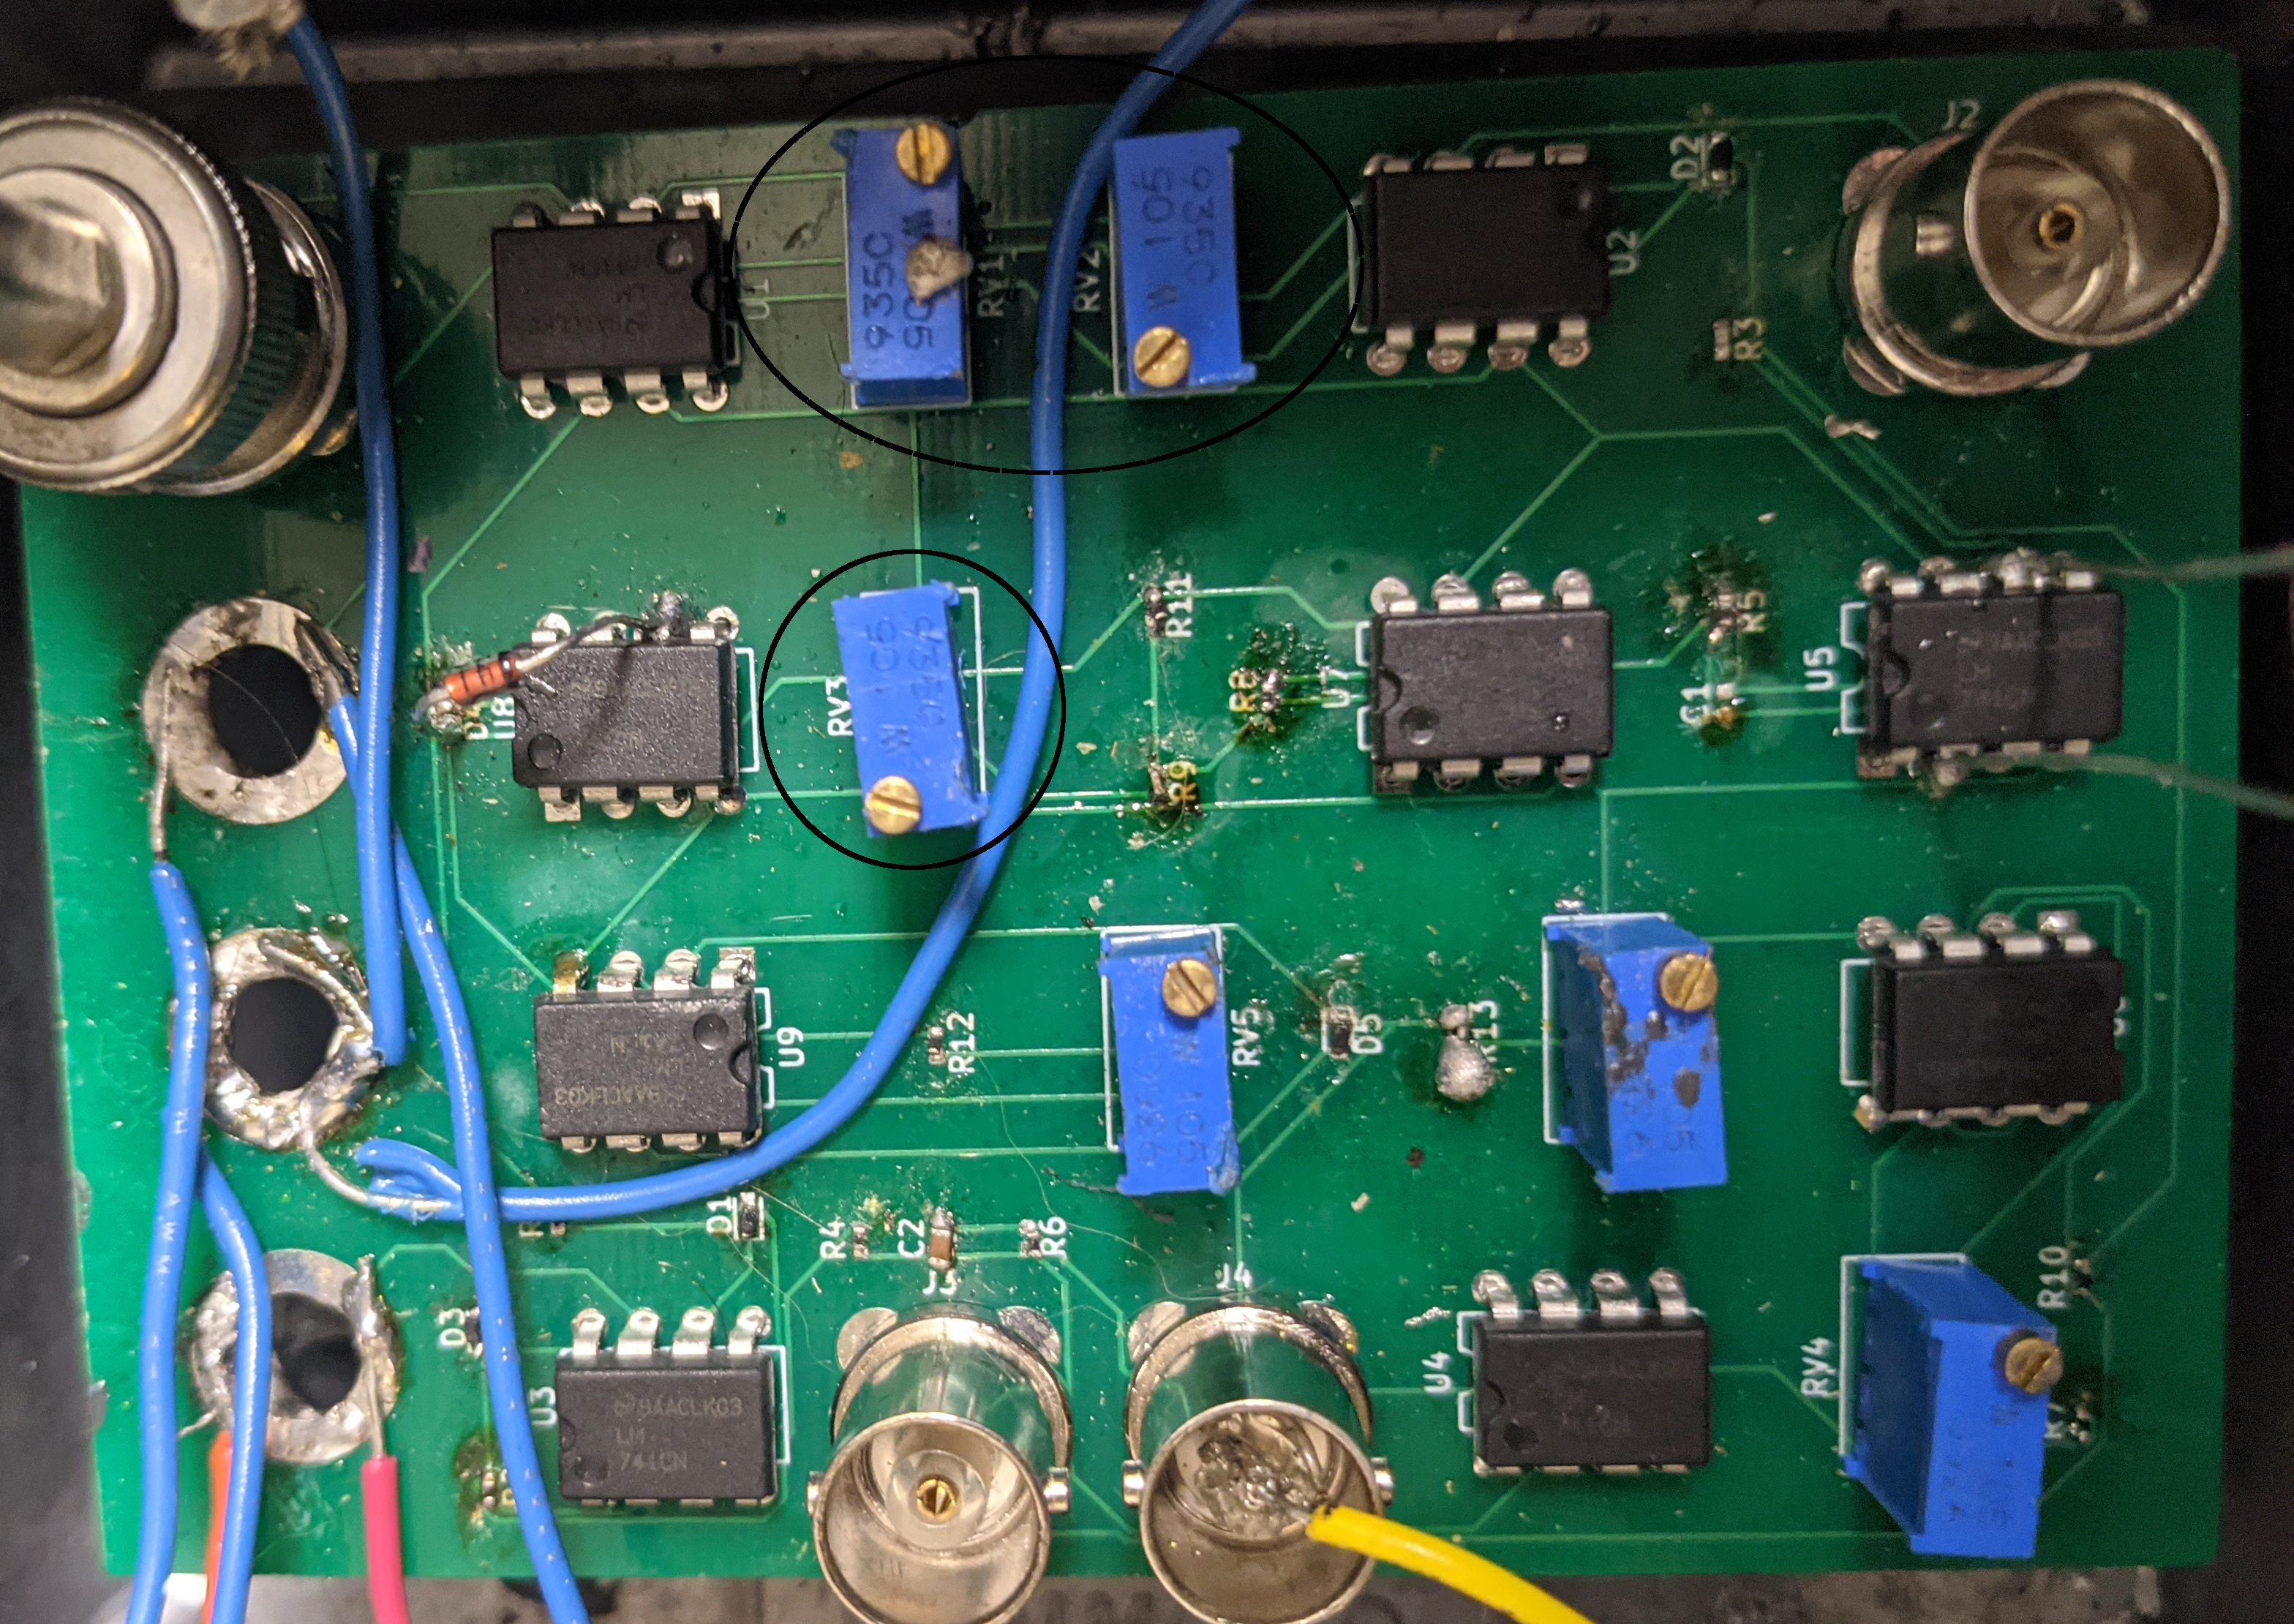
\includegraphics[width=0.6\textwidth]{Data for Probe Writeup/circuit.jpg}
	\caption{Response at 76 kHz.}
\end{figure}

\section{Control programs for fixed background}\label{controlprograms}
\hypertarget{controlprograms}{}

\par{}

\begin{figure}[!h]
	\centering
	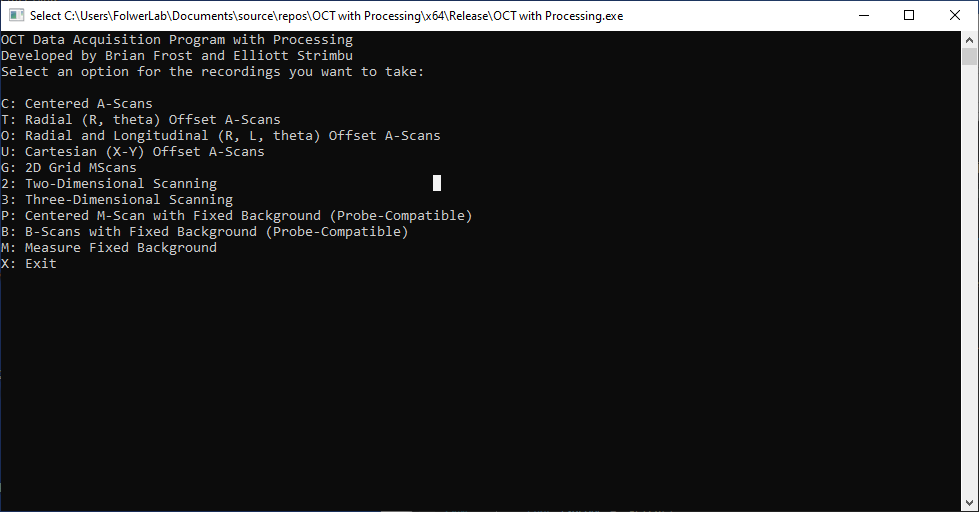
\includegraphics[width=0.6\textwidth]{Data for Probe Writeup/Terminal at Startup.png}
	\caption{.}
\end{figure}

\subsection{Option M: Measure Background}

\par{}

\begin{figure}[!h]
	\centering
	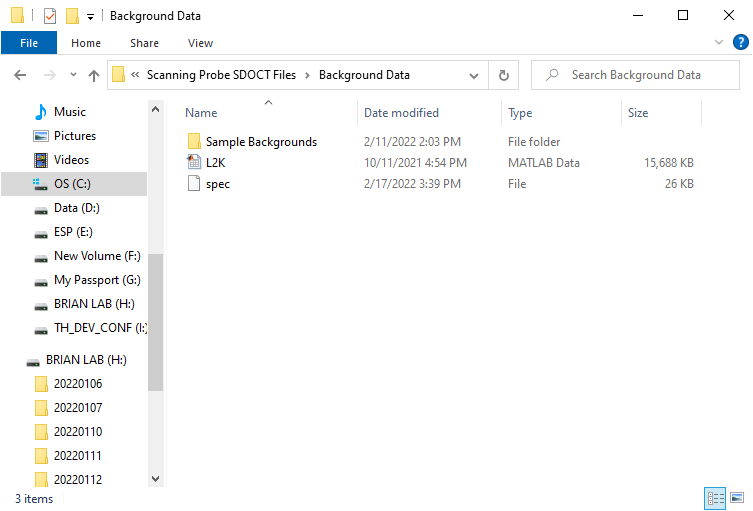
\includegraphics[width=0.6\textwidth]{Data for Probe Writeup/spec location.png}
	\caption{.}
\end{figure}

\subsection{Taking and observing B-Scans with fixed background}

\par{}

\begin{figure}[!h]
	\centering
	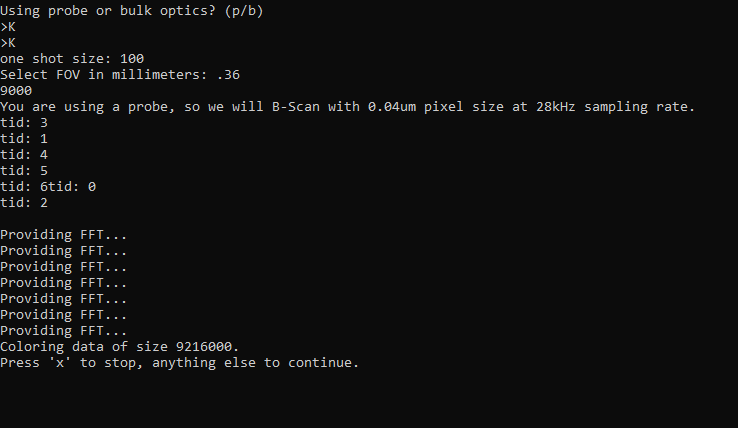
\includegraphics[width=0.6\textwidth]{Data for Probe Writeup/BMode Probe.png}
	\caption{.}
\end{figure}

\begin{figure}[!h]
	\centering
	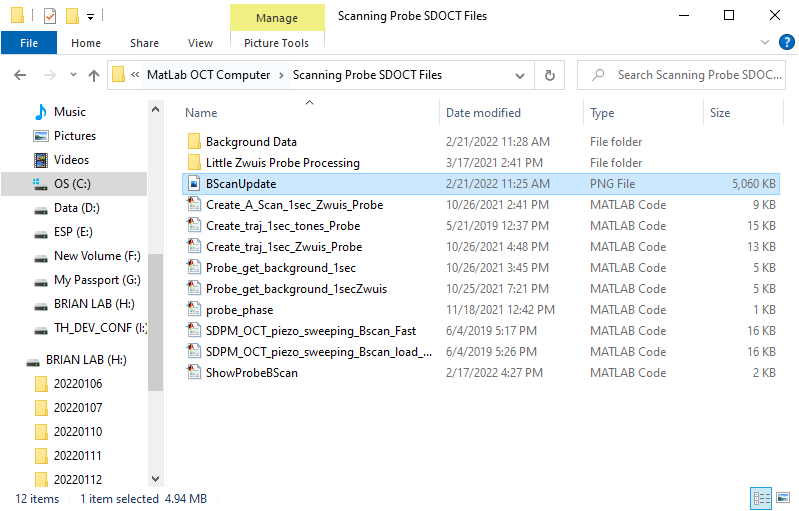
\includegraphics[width=0.6\textwidth]{Data for Probe Writeup/BScan location.png}
	\caption{.}
\end{figure}

\begin{figure}[!h]
	\centering
	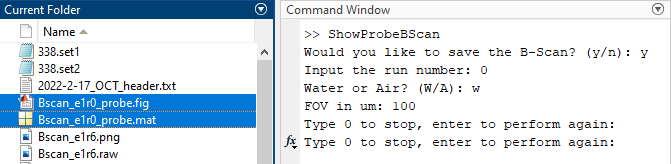
\includegraphics[width=0.6\textwidth]{Data for Probe Writeup/ShowProbeBScan operation.png}
	\caption{.}
\end{figure}

\begin{figure}[!h]
	\centering
	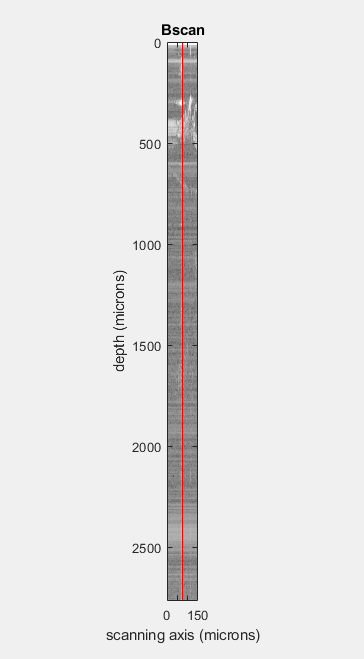
\includegraphics[width=0.6\textwidth]{Data for Probe Writeup/BScan fig update.png}
	\caption{.}
\end{figure}

\subsection{Option P: M-Scans with fixed background}

\par{}

\section{Using ThorImage with the probe}\label{thorimagesection}
\hypertarget{thorimagesection}{}

\par{}


\begin{figure}[!h]
	\centering
	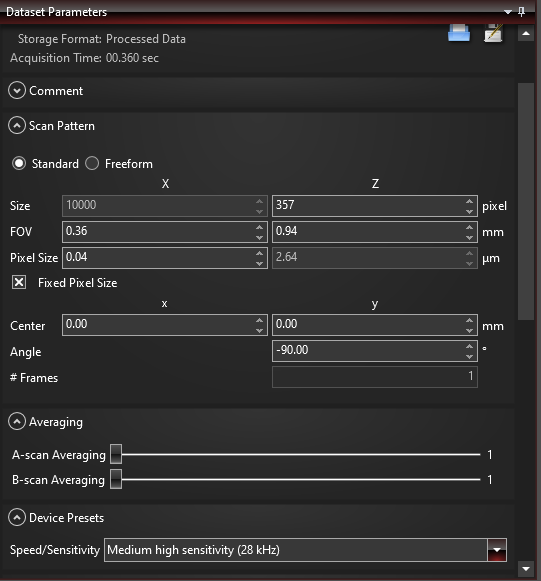
\includegraphics[width=0.6\textwidth]{Data for Probe Writeup/ThorImage settings for BScan.png}
	\caption{.}
\end{figure}


\subsection{The ThorImage ``fake background" trick}

\par{}

\section{Signal quality}

\par{}

\subsection{SNR in air vs. water}\label{SNRsection}
\hypertarget{SNRsection}{}

\par{}

\begin{figure}[!h]
	\centering
	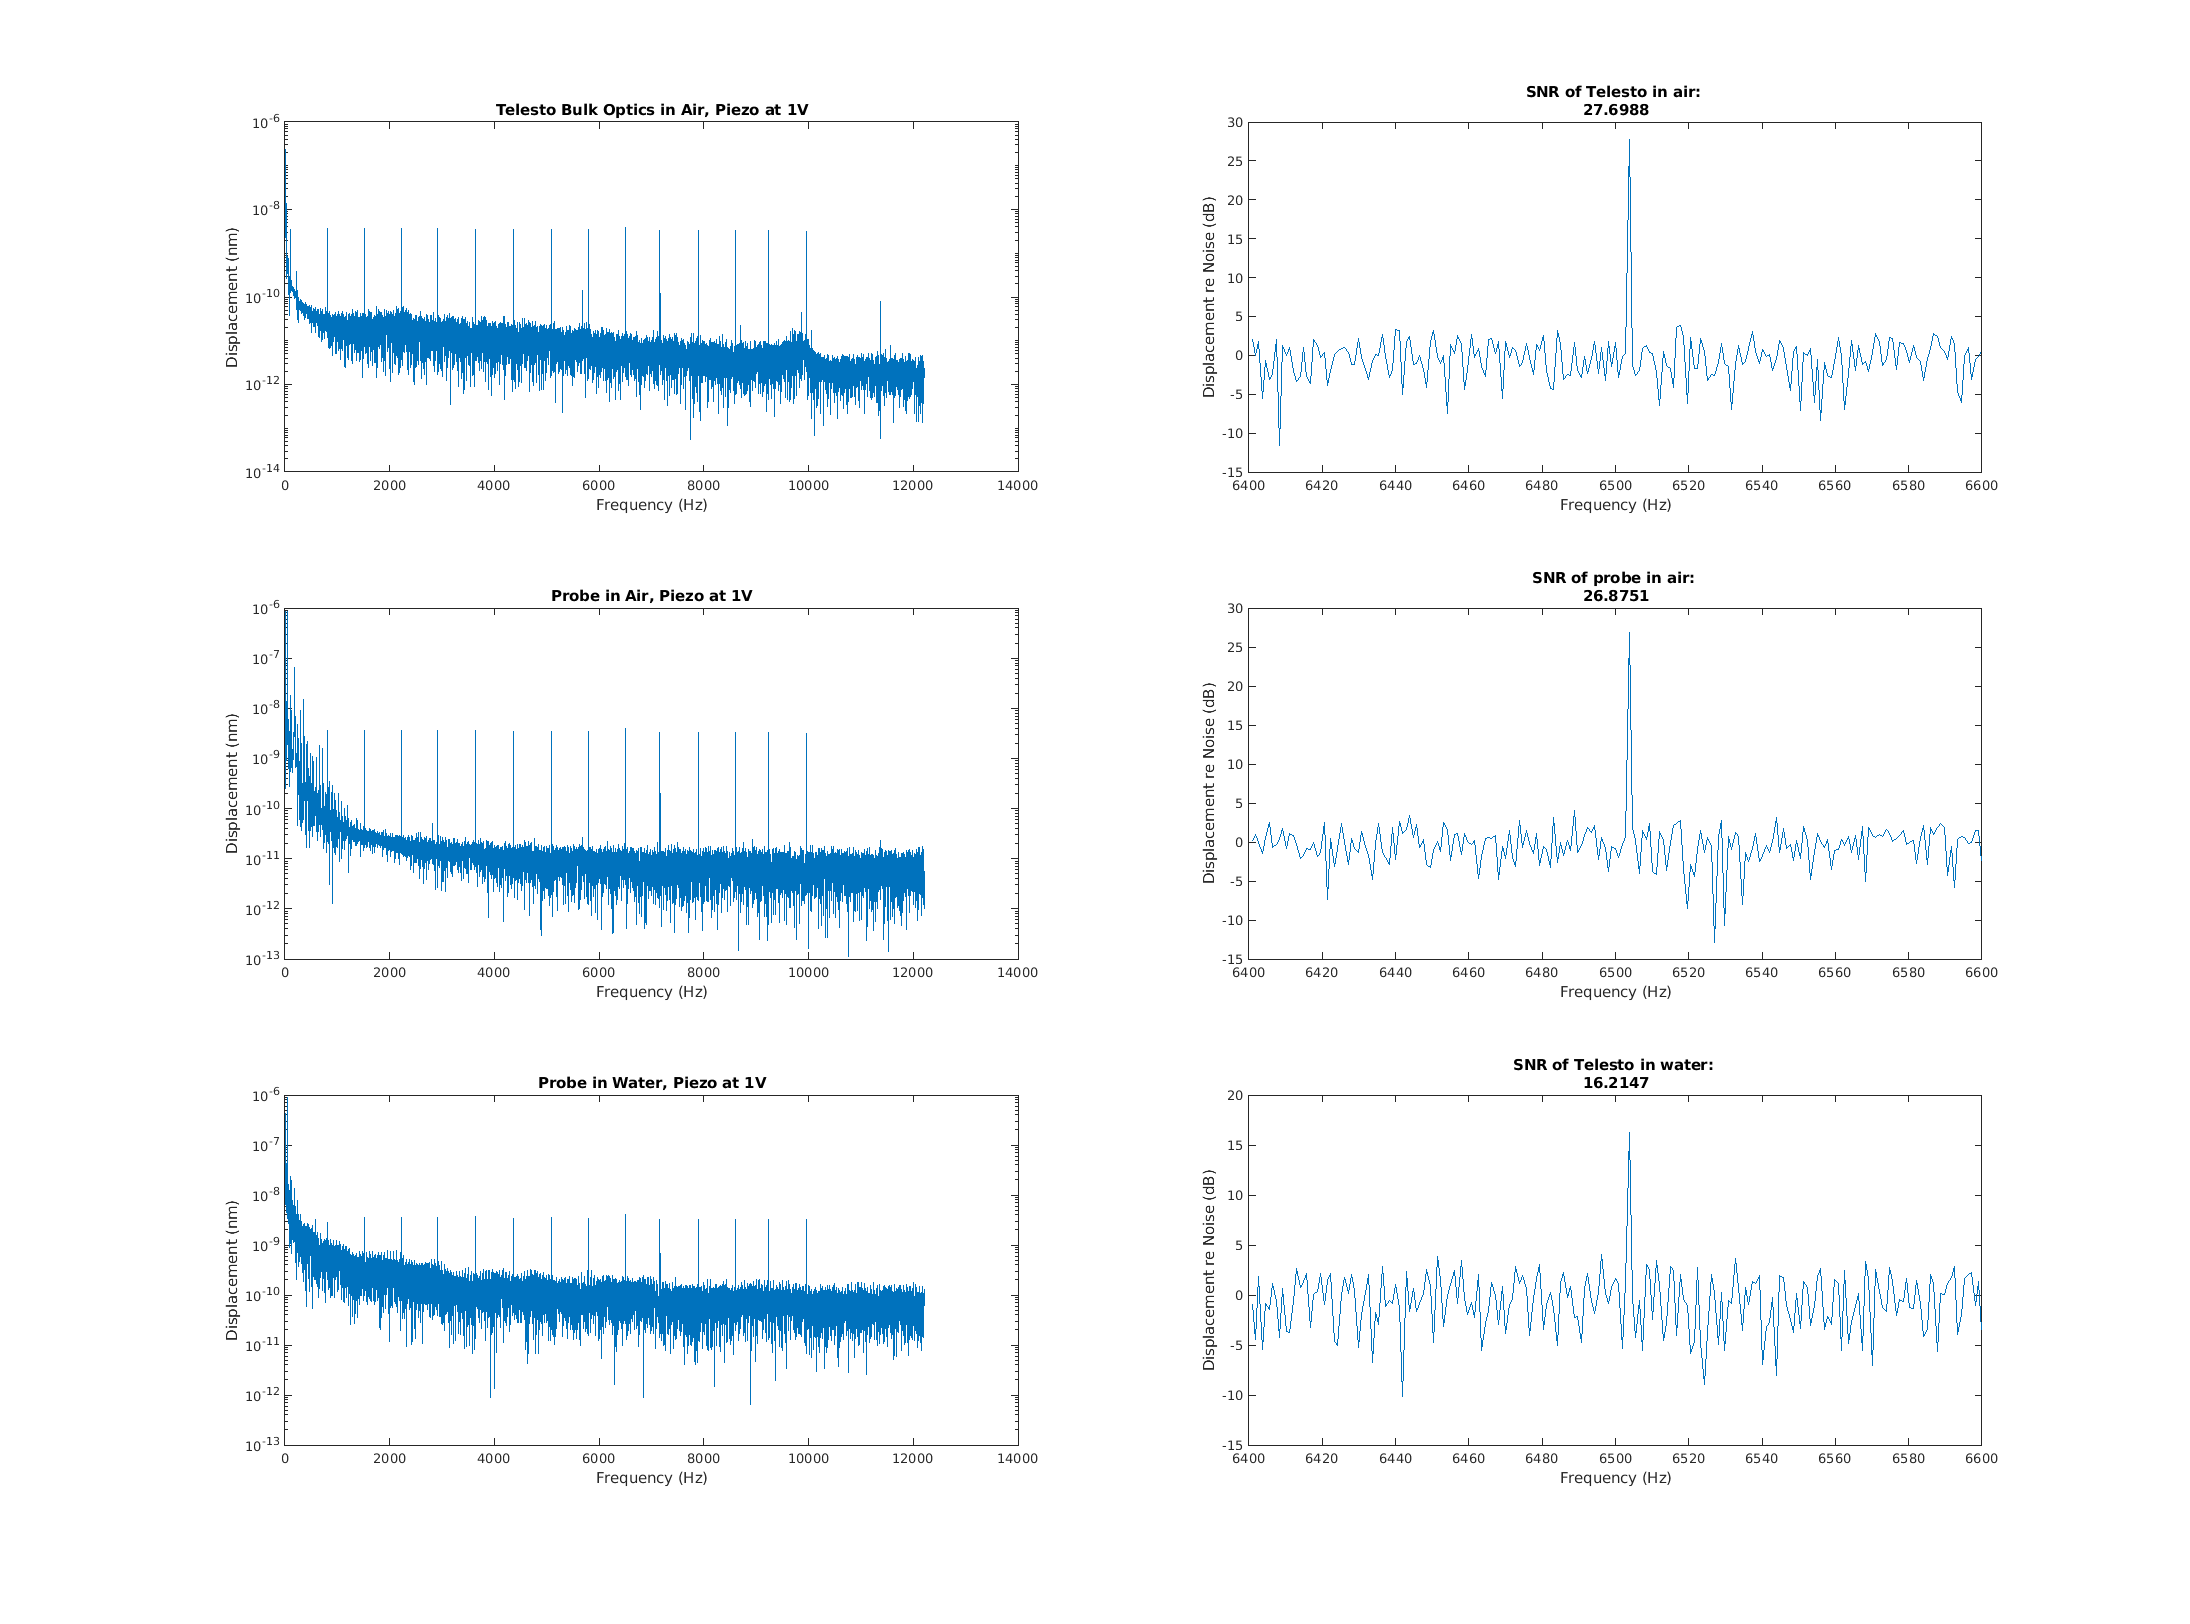
\includegraphics[width=\textwidth]{Data for Probe Writeup/SNRcomp.png}
	\caption{.}
\end{figure}

\subsection{B-Scan quality}\label{BScansection}
\hypertarget{BScansection}{}

\par{}

\begin{figure}[!h]
	\centering
	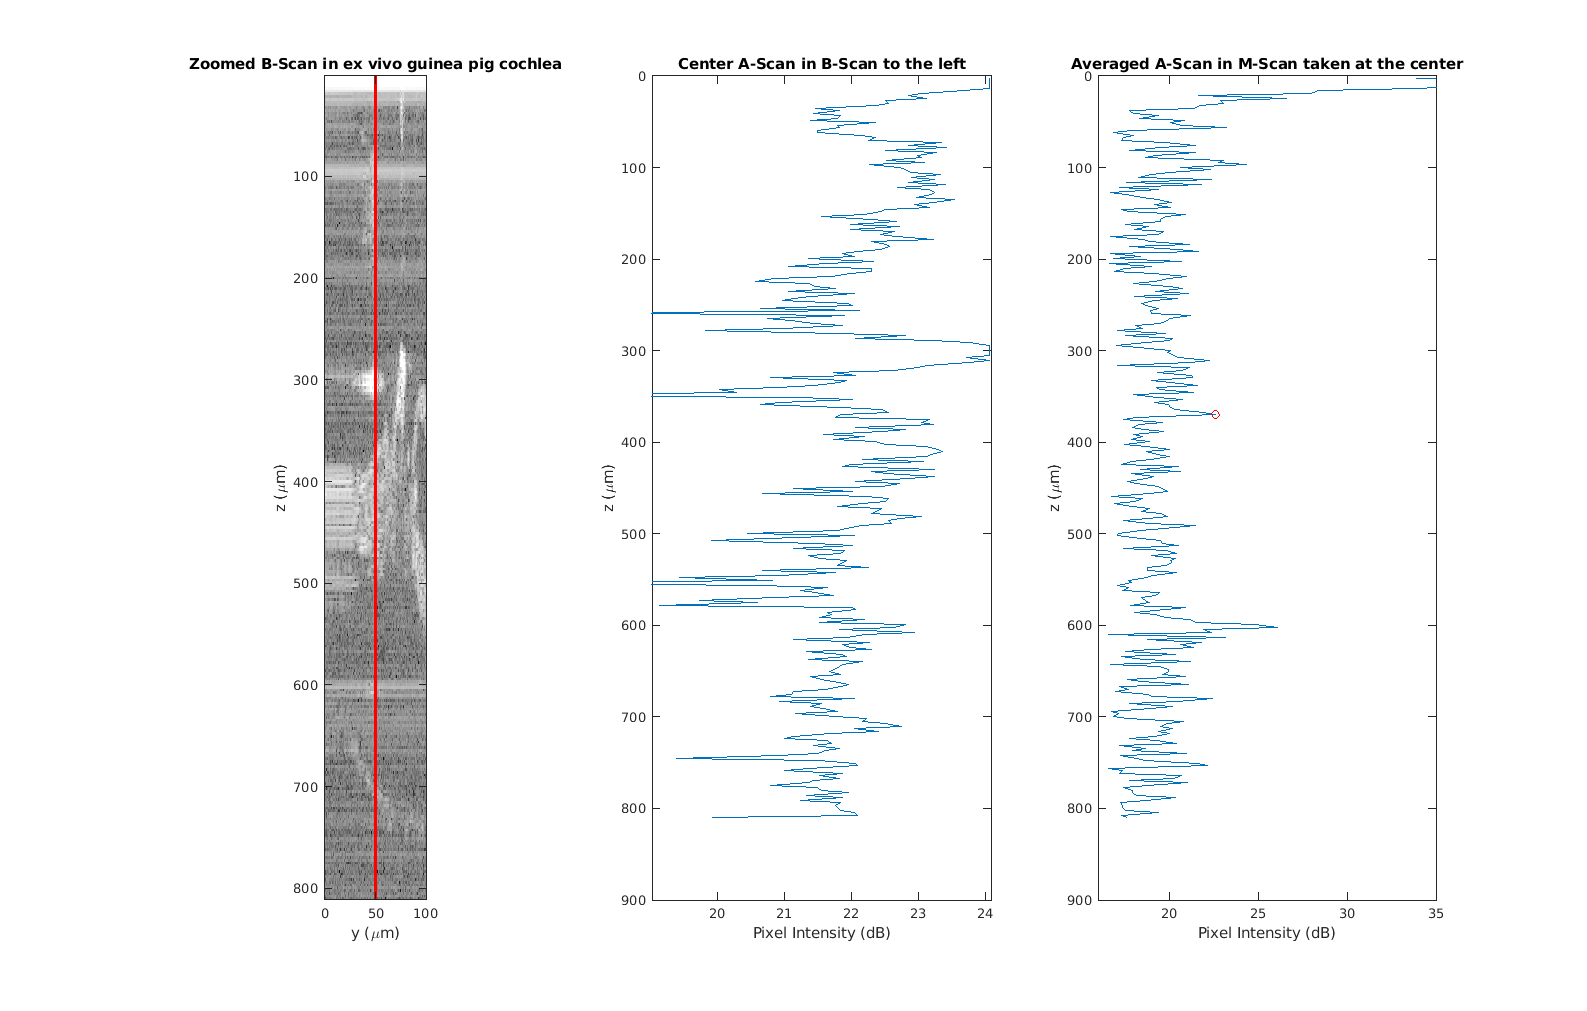
\includegraphics[width=\textwidth]{Data for Probe Writeup/Data 2022-2-17/BScan v AScan.png}
	\caption{.}
\end{figure}


\end{document}
